\lab{Linear Systems}{Linear Systems}
\objective{The fundamental problem of linear algebra is solving the linear system $A\x = \b$, if it is even possible.
There are many approaches to solving this problem, each with different pros and cons.
In this lab we implement the LU Decomposition and use it to solve square linear systems.
We also introduce SciPy, together with its libraries for linear algebra and working with sparse matrices.
}

\section*{Gaussian Elimination} % =============================================

The standard approach for solving the linear system $A\x = b$ on paper is reducing the augmented matrix $\left[A\mid\b\right]$ to row-echelon form (REF) via \emph{Gaussian elimination}, then using back substitution.
The matrix is in REF when the leading non-zero term in each row is the diagonal term, so the matrix is upper triangular.

At each step of the process, there are three possible operations: swapping two rows, multiplying one row by a scalar value, or adding a scalar multiple of one row to another.
Many systems, like the one displayed below, can be reduced to REF using only the third type of operation.
First we use multiples of the first row to get zeros below the diagonal in the first column, then we use a multiple of the second row to get zeros below the diagonal in the second column.
%
\begin{align*}
\left[\begin{array}{ccc|c}
1 & 1 & 1 & 1 \\
1 & 4 & 2 & 3 \\
4 & 7 & 8 & 9 \\
\end{array}\right]
\longrightarrow
\left[\begin{array}{ccc|c}
1 & 1 & 1 & 1 \\
\textcolor{red}0 & 3 & 1 & 2 \\
4 & 7 & 8 & 9 \\
\end{array}\right]
\longrightarrow
\left[\begin{array}{ccc|c}
1 & 1 & 1 & 1 \\
0 & 3 & 1 & 2 \\
\textcolor{red}0 & 3 & 4 & 5 \\
\end{array}\right]
\longrightarrow
\left[\begin{array}{ccc|c}
1 & 1 & 1 & 1 \\
0 & 3 & 1 & 2 \\
0 & \textcolor{red}0 & 3 & 3
\end{array}\right]
\end{align*}

Each of these operations is mathematically equivalent to left-multiplying by a \emph{type III elementary matrix}, the identity with one non-diagonal non-zero term.
If row operation $k$ corresponds to matrix $E_k$, the following equation is $E_3E_2E_1A = U$.
%
\begin{align*}
\left[\begin{array}{ccc}
1 & 0 & 0 \\
0 & 1 & 0 \\
0 & -1 & 1 \\
\end{array}\right]
\left[\begin{array}{ccc}
1 & 0 & 0 \\
0 & 1 & 0 \\
-4 & 0 & 1 \\
\end{array}\right]
\left[\begin{array}{ccc}
1 & 0 & 0 \\
-1 & 1 & 0 \\
0 & 0 & 1 \\
\end{array}\right]
\left[\begin{array}{ccc|c}
1 & 1 & 1 & 1 \\
1 & 4 & 2 & 3 \\
4 & 7 & 8 & 9 \\
\end{array}\right]
=
\left[\begin{array}{ccc|c}
1 & 1 & 1 & 1 \\
0 & 3 & 1 & 2 \\
0 & 0 & 3 & 3
\end{array}\right]
\end{align*}

However, matrix multiplication is an inefficient way to implement row reduction.
Instead, modify the matrix \emph{in place} (without making a copy), changing only those entries that are affected by each row operation.

\begin{lstlisting}
>>> import numpy as np
>>> A = np.array([[1, 1, 1, 1],
...               [1, 4, 2, 3],
...               [4, 7, 8, 9]], dtype=np.float)

# Reduce the 0th column to zeros below the diagonal.
>>> A[1,0:] -= (A[1,0] / A[0,0]) * A[0]
>>> A[2,0:] -= (A[2,0] / A[0,0]) * A[0]

# Reduce the 1st column to zeros below the diagonal.
>>> A[2,1:] -= (A[2,1] / A[1,1]) * A[1,1:]
>>> print A
[[ 1.  1.  1.  1.]
 [ 0.  3.  1.  2.]
 [ 0.  0.  3.  3.]]
\end{lstlisting}

Note that the final row operation modifies only part of the third row to avoid spending the computation time of adding $0$ to $0$.

If a $0$ appears on the main diagonal during any part of row reduction, the approach given above tries to divide by $0$.
When this happens, swap the current row with one below it that does not have a $0$ in the same column.
This is equivalent to left-multiplying by a type II elementary matrix, also called a \emph{permutation matrix}.

\begin{problem} % Program simple row reduction to REF.
Write a function which reduces a \textbf{square} matrix $A$ to REF.
You may assume that $A$ is invertible and that a $0$ will never appear on the main diagonal (so only use type III row reductions, not type II).
Avoid operating on entries that you know will be $0$ before and after a row operation.

Consider generating small random matrices as test cases with NumPy's \li{random} module (\li{np.random.randint()} may be particularly useful).
\label{prob:ref-row-reduction}
\end{problem}

\begin{warn} % Gaussian Elimination is numerically unstable!
Gaussian elimination is not always numerically stable.
Suppose that, due to roundoff error, we have a matrix with a very small entry on the diagonal.

\begin{align*}
A = \left[\begin{array}{cc}
10^{-15} & 1 \\
-1 & 0 \\
\end{array}\right]
\end{align*}

$10^{-15}$ is essentially zero, but instead of swapping the first and second rows to put the $A$ in REF, a computer might multiply the first row by $10^{15}$ and add it to the second row to eliminate the $-1$.
The resulting matrix is far from what we would expect on paper.

\begin{align*}
\left[\begin{array}{cc}
10^{-15} & 1 \\
-1 & 0 \\
\end{array}\right]
\longrightarrow
\left[\begin{array}{cc}
10^{-15} & 1 \\
0 & 10^{15} \\
\end{array}\right]
\end{align*}

Round-off error can propagate through many steps in a calculation, resulting in garbage output.
NumPy's routines that employ row reduction use several tricks to minimize the impact of round-off errors, but beware that these tricks can't fix every matrix.
\end{warn}

\subsection*{The LU Decomposition} % ------------------------------------------

The \emph{LU decomposition} of a square matrix $A$ is a factorization $A=LU$ where $U$ is the \textbf{upper} triangular REF of $A$ and $L$ is the \textbf{lower} triangular product of the type III elementary matrices whose inverses reduce $A$ to $U$.
% Thus, the LU decomposition is an efficient way of storing the REF and how we got there.
The LU decomposition of $A$ exists when $A$ can be reduced to REF using only type III elementary matrices (no row swaps).
However, the rows of $A$ can always be permuted in a way such that the decomposition exists.
If $P$ is a permutation matrix encoding the appropriate row swaps, then the decomposition $PA = LU$ always exists.

Suppose $A$ has an LU decomposition (not requiring row swaps).
Then $A$ can be reduced to REF with $k$ row operations, corresponding to left-multiplying the type III elementary matrices $E_1, \ldots, E_k$.
% Then $U = E_k \ldots E_2E_1A,$ where $U$ is the REF of $A$.
Because there were no row swaps, each $E_i$ is lower triangular, so each inverse $E_i^{-1}$ is also lower triangular.
Furthermore, since the product of lower triangular matrices is lower triangular, $L$ is lower triangular.
%
\begin{align*}
E_k\ldots E_2E_1 A = U\quad \longrightarrow\quad A &= (E_k \ldots E_2E_1)^{-1} U \\
&= E_1^{-1}E_2^{-1}\ldots E_k^{-1}U \\
&= LU
\end{align*}

We can thus compute $L$ by right-multiplying the identity by the matrices we used to reduce $U$.
However, in this special situation, each right-multiplication only changes one entry of $L$, so we can avoid matrix multiplication altogether.
The entire process, only slightly different than row reduction, is summarized below. % in Algorithm \ref{alg:LU-Decomposition}.
%
\begin{algorithm}[H]
\begin{algorithmic}[1]
\Procedure{LU Decomposition}{$A$}
\State $U \gets A$ (make a copy of $A$ with \li{np.copy()})
\State $L \gets I$ (the $n\times n$ identity matrix)
\For{$j=0 \ldots n-1$}
    \For{$i=j+1 \ldots m-1$}
        \State $L_{i,j} \gets U_{i, j}/U_{j, j}$
        \State $U_{i,j:} \gets U_{i,j:} - L_{i,j}U_{j,j:}$
    \EndFor
\EndFor
\State \pseudoli{return} $L, U$
\EndProcedure
\end{algorithmic}
\caption{}
\label{alg:LU-Decomposition}
\end{algorithm}

\begin{problem}
Write a function that finds the LU decomposition of a square matrix.
You may assume the decomposition exists and requires no row swaps.
\label{prob:LU-Decomposition}
\end{problem}

\subsection*{Forward and Backward Substitution} % -----------------------------

If $A\x = \b$ and $PA = LU$, then $LU\x = PA\x = P\b$.
We can solve this system by first solving $L\y = P\b$, then $U\x = \y$.
Since $L$ and $U$ are both triangular, these systems can be solved with backward and forward substitution.
We can thus compute the $LU$ factorization of $A$ once, then use substitution to efficiently solve $A\x=\b$ for various values of $\b$.
% This technique is significantly faster than storing $A^{-1}$ and then computing $A^{-1}\b$ (see Problem \ref{prob:solve}).

The square, triangular system $L\y = \b$ has the following form:
%
\begin{align*}
\left[\begin{array}{ccccc}
1      & 0      & 0      & \cdots & 0 \\
l_{21} & 1      & 0      & \cdots & 0 \\
l_{31} & l_{32} & 1      & \cdots & 0 \\
\vdots & \vdots & \vdots & \ddots & \vdots \\
l_{n1} & l_{n2} & l_{n3} & \cdots & 1
\end{array}\right]
\left[\begin{array}{c}
y_1 \\ y_2 \\ y_3 \\ \vdots \\ y_n \\
\end{array}\right]
=
\left[\begin{array}{c}
b_1 \\ b_2 \\ b_3 \\ \vdots \\ b_n \\
\end{array}\right]
\end{align*}

Matrix multiplication yields the following equations:
%
\begin{align}
\nonumber y_1 &= b_1 & y_1 &= b_1 \\
\nonumber l_{21}y_1 + y_2 &= b_2 & y_2 &= b_2 - l_{21}y_1 \\
% \nonumber l_{31}y_1 + l_{21}y_2 + y_3 &= b_3 & y_3 &= b_3 - l_{31}y_1 - l_{32}y_2 \\
\nonumber & \vdots & \vdots & \\
\sum_{j=1}^{k-1}l_{kj}y_j + y_k &= b_k & y_k &= b_k - \sum_{j=1}^{k-1}l_{kj}y_j
\label{eq:forward-substitution}
\end{align}

The triangular system $U\x = \b$ yields similar equations, but in reverse order:
%
\begin{align*}
\left[\begin{array}{ccccc}
u_{11} & u_{12} & u_{13} & \cdots & u_{1n} \\
0      & u_{22} & u_{23} & \cdots & u_{2n} \\
0      & 0      & u_{33} & \cdots & u_{3n} \\
\vdots & \vdots & \vdots & \ddots & \vdots \\
0      & 0      & 0      & \cdots & u_{nn}
\end{array}\right]
\left[\begin{array}{c}
x_1 \\ x_2 \\ x_3 \\ \vdots \\ x_n \\
\end{array}\right]
=
\left[\begin{array}{c}
y_1 \\ y_2 \\ y_3 \\ \vdots \\ y_n \\
\end{array}\right]
\end{align*}
%
\begin{align}
\nonumber u_{nn}x_n &= y_n & x_n &= \frac{1}{u_{nn}}y_n \\
\nonumber u_{n-1,n-1}x_{n-1} + u_{n-1,n}x_{n} &= y_{n-1} & x_{n-1} &= \frac{1}{u_{n-1,n-1}}\left(y_{n-1} - u_{n-1,n}x_{n}\right)\\
\nonumber & \vdots & \vdots & \\
\sum_{j=k}^{n}u_{kj}x_j &= y_k & x_k &= \frac{1}{u_{kk}}\left(y_k - \sum_{j=k+1}^{n}u_{kj}x_j\right)
\label{eq:backward-substitution}
\end{align}

\begin{problem} % Program back and forward substitution.
Write a function that, given $A$ and $\b$, solves the square linear system $A\x = \b$.
Use the function from Problem \ref{prob:LU-Decomposition} to compute $L$ and $U$, then use Equations \ref{eq:forward-substitution} and \ref{eq:backward-substitution} to solve for $\y$, then $\x$.
You may again assume that there are no row swaps (so $P = I$ in this case).
\label{prob:substitute-solve}
\end{problem}

\section*{SciPy} % ============================================================

SciPy is a powerful scientific computing library built upon NumPy.
It includes high-level tools for linear algebra, statistics, signal processing, integration, optimization, machine learning, and more.
% We typically import SciPy with the convention \li{import scipy as sp}.

\subsection*{Linear Algebra} % ------------------------------------------------

NumPy and SciPy both have a linear algebra module, each called \li{linalg}, but SciPy's module is the larger of the two.
Some of SciPy's common \li{linalg} functions are listed below.
See \url{http://docs.scipy.org/doc/scipy/reference/linalg.html} for more documentation.
%
\begin{table}[H]
\centering
\begin{tabular}{r|l}
    Function & Returns \\ \hline
    \li{det()} & The determinant of a square matrix. \\
    \li{eig()} & The eigenvalues and eigenvectors of a square matrix. \\
    \li{inv()} & The inverse of an invertible matrix. \\
    \li{norm()} & The norm of a vector or matrix norm of a matrix. \\
    \li{solve()} & The solution to $A\x = \b$ (the system may not be square).
\end{tabular}
\end{table}

This library also includes routines for computing matrix decompositions.

\begin{lstlisting}
>>> from scipy import linalg as la

# Make a random matrix and a random vector.
>>> A = np.random.random((1000,1000))
>>> b = np.random.random(1000)

# Compute the LU decomposition of A, including pivots.
>>> lu, piv = la.lu_factor(A)

# Use the LU decomposition to solve Ax = b.
>>> x = la.lu_solve((lu,piv), b)

# Check that the solution is legitimate.
>>> np.allclose(A.dot(x), b)
True
\end{lstlisting}

As with NumPy, SciPy's routines are all highly optimized.
However, some algorithms are, by nature, faster than others.

\begin{problem} % Time ways to solve Ax = b with scipy.linalg.
Write a function that times different \li{scipy.linalg} functions for solving square linear systems.

For various values of $n$, generate a random $n \times n$ matrix $A$ and a random $n \times 1$ vector $\b$ using \li{np.random.random()}.
Time how long it takes to solve the system $A\x = \b$ with each of the following approaches:
%
\begin{itemize}
\item Invert $A$ with \li{la.inv()} and left-multiply the inverse to $\b$.
\item Use \li{la.solve()}.
\item Use \li{la.lu_factor()} and \li{la.lu_solve()} to solve the system with the LU decomposition.
\item Use \li{la.lu_factor()} and \li{la.lu_solve()}, but only time \li{la.lu_solve()}.
\end{itemize}
%
Plot the system size $n$ versus the execution times.
Use log scales if needed.
\end{problem}

\begin{info}
Numerically inverting matrices is so costly that there is hardly ever a good reason to do it.
Use a specific solver, like \li{la.lu_solve()}, whenever possible.
\end{info}

\subsection*{Sparse Matrices} % -----------------------------------------------

Large linear systems can have tens of thousands of parameters.
Storing the corresponding matrices in memory can be difficult: a $100000 \times 100000$ system requires around 40 GB to store in a NumPy array (4 bytes per entry $\times\ 10^{10}$ entries).
This is well beyond the amount of RAM in a normal laptop.

In applications where systems of this size arise, it is common that such matrices are \emph{sparse}, meaning that most of the entries are $0$.
% Taking advantage of the sparse structure of these matrices uses less memory and decreases computation time.
SciPy's \li{sparse} module provides tools for efficiently constructing and manipulating 1- and 2-D sparse matrices.
A \li{sparse} matrix only stores the nonzero values and the positions of these values.
For sufficiently sparse matrices, storing the matrix as a \li{sparse} matrix may only take megabytes, rather than gigabytes.

For example, diagonal matrices are sparse.
Storing an $n \times n$ diagonal matrix in the na\"{i}ve way means storing $n^2$ values in memory.
It is almost always more efficient to instead store the diagonal entries in a 1-D array of $n$ values.
In addition to using less storage space, this allows for much faster matrix operations: the standard algorithm to multiply a matrix by a diagonal matrix involves $n^3$ steps, but most of these are multiplying by or adding $0$.
A smarter algorithm can accomplish the same task much faster.

% \subsection*{Types of Sparse Matrices} % -----------------------------------

SciPy has seven \li{sparse} matrix types, listed below.
Each type is optimized either for storing sparse matrices whose nonzero entries follow certain patterns, or for performing certain computations.

\begin{table}[H]
\centering
\begin{tabular}{c|l|l}
    Name & \multicolumn{1}{c|}{Description} & \multicolumn{1}{c}{Advantages}
    \\ \hline
    \li{bsr_matrix} & Block Sparse Row & Specialized structure. \\
    \li{coo_matrix} & Coordinate Format & Conversion among sparse formats. \\
    \li{csc_matrix} & Compressed Sparse Column & Column-based operations and slicing.\\
    \li{csr_matrix} & Compressed Sparse Row & Row-based operations and slicing. \\
    \li{dia_matrix} & Diagonal Storage & Specialized structure. \\
    \li{dok_matrix} & Dictionary of Keys & Element access, incremental construction. \\
    \li{lil_matrix} & Row-based Linked List & Incremental construction. \\
                    &                & Conversion to CSR or CSC format. \\
\end{tabular}
\end{table}

\subsubsection*{Creating Sparse Matrices} % -----------------------------------

A regular, non-sparse matrix is called \emph{full} or \emph{dense}.
Full matrices can be converted to each of the sparse matrix formats listed above.
However, it is more memory efficient to never create the full matrix in the first place.
There are really three different approaches for creating sparse matrices from scratch.

\begin{itemize}

\item \textbf{Coordinate Format}:
When all of the nonzero values and their positions are known, create the entire sparse matrix at once as a \li{coo_matrix}.
All nonzero values are stored as a location (or coordinate) and value.
This format also supports very fast conversion between the other sparse matrix types.

\begin{lstlisting}
>>> from scipy import sparse

# Define the rows, columns, and values separately.
>>> rows = np.array([0, 1, 0])
>>> cols = np.array([0, 1, 1])
>>> vals = np.array([3, 5, 2])
>>> A = sparse.coo_matrix((vals, (rows,cols)), shape=(3,3))
>>> print(A)
  (0, 0)    3
  (1, 1)    5
  (0, 1)    2

# The toarray() method casts the sparse matrix as a NumPy array.
# However, using regular arrays forfeits all sparse-related optimizations.
>>> print(A.toarray())
[[3 2 0]
 [0 5 0]
 [0 0 0]]
\end{lstlisting}

\item \textbf{DOK and LIL Formats}:
If the matrix values and their locations are not known a priori, construct the matrix incrementally with \li{dok_matrix} or \li{lil_matrix}.
Indicate the size of the matrix, then change individual values with regular slicing syntax.
This method is quite similar syntactically to NumPy.

\begin{lstlisting}
>>> B = sparse.lil_matrix((2,6))
>>> B[0,2] = 4
>>> B[1,4] = 9

>>> print(B.toarray())
[[ 0.  0.  4.  0.  0.  0.]
 [ 0.  0.  0.  0.  9.  0.]]
\end{lstlisting}

% OLD VERSION
\begin{comment}
A second way to create a sparse matrix is to pre-allocate an array of zeros and then specify the nonzero entries one at a time.
The most efficient sparse matrix types for building matrices incrementally are \li{lil_matrix} and \li{dok_matrix}.
Once you are done constructing the sparse matrix, you should convert it to a form that is optimized for computations.

\begin{lstlisting}
# Initialize Z.
>>> Z = sparse.lil_matrix((400, 300))
# Specify the nonzero entries of Z.
>>> Z[1,34] = 23
>>> Z[23,32] = 56
>>> Z[2,:] = 13.2
>>> Z
<400x300 sparse matrix of type '<type 'numpy.float64'>'
  with 302 stored elements in LInked List format>
\end{lstlisting}

When the matrix \li{Z} is initialized, all its entries are assumed to be zero.
Note that at the end of \li{Z}'s construction, only 302 elements are being stored for a matrix with $120000$ entries.

The only way to view a matrix as a 2-D array is to convert it to a full matrix.
If your matrix is too large to do this, you can still visualize it using the \li{plt.spy()} command from matplotlib.
This function plots the locations of the non-zero entries in a matrix.
The following code outputs Figure \ref{fig:mpl_spy}.

\begin{lstlisting}
>>> from matplotlib import pyplot as plt
>>> B = np.random.rand(3, 10000)
>>> A = sparse.spdiags(B, [-1, 0, 1], 10000, 10000)
>>> plt.spy(A)
\end{lstlisting}

\begin{figure}
\centering
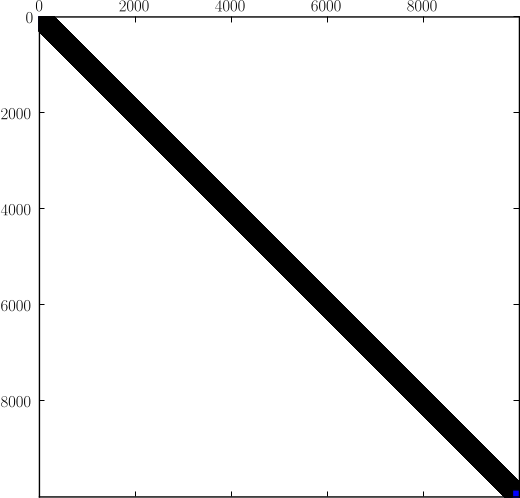
\includegraphics[width=.7\textwidth]{spy.png}
\caption{}
\label{fig:mpl_spy}
\end{figure}
\end{comment}

\item \textbf{DIA and BSR Formats}:
When the matrix has a particular sparsity pattern, such as nonzero blocks or diagonals, use \li{bsr_matrix} or \li{dia_matrix}.

% % spdiags() for some reason?
Use the method \li{sparse.spdiags(data, diags, m, n)}.
If \li{data} is a 1-D array and \li{diags} is a scalar, then this method creates an $m \times n$ matrix with \li{data} on the specified diagonal.
The parameter \li{diags=0} indicates the main diagonal, with lower diagonals indexed by negative numbers and upper diagonals by positive numbers.
If \li{data} is a 2-D array and \li{diags} is a list, then this method creates an $m \times n$ matrix with the rows of \li{data} on the diagonals specified by \li{diags}.

\begin{lstlisting}
# Create a sparse 3x3 matrix with (2, 3, 4) on the diagonal.
>>> A = sparse.spdiags([2, 3, 4], 0, 3, 3)
>>> A
<<<3x3 sparse matrix of type '<type 'numpy.int64'>'
  with 3 stored elements (1 diagonals) in DIAgonal format>>>
# Convert A to a full matrix.
>>> print(A.toarray())
[[2, 0, 0],
 [0, 3, 0],
 [0, 0, 4]]

# Create a sparse 4x4 matrix with the rows of diag_entries on the diagonals.
>>> diag_entries = np.array([[3,6,9,0],[1,4,7,10],[0,2,5,8]])
>>> B = sparse.spdiags(diag_entries, [-1, 0, 1], 4, 4)
>>> B
<<<4x4 sparse matrix of type '<type 'numpy.int64'>'
  with 10 stored elements (3 diagonals) in DIAgonal format>>>
>>> print(B.toarray())
[[ 1,  2,  0,  0],
 [ 3,  4,  5,  0],
 [ 0,  6,  7,  8],
 [ 0,  0,  9, 10]]
\end{lstlisting}

\end{itemize}

\begin{info} % Note about banded matrices.
The final matrix $B$ in the example above is called a \emph{banded} matrix.
A banded matrix is a sparse matrix whose only non-zero entries are on the main diagonal and on some diagonals on either side.
In fact, $B$ is an example of a \emph{tri-diagonal} matrix, because its nonzero entries are confined to the three central diagonals.
Banded matrices arise naturally in many applications, including numerical methods for solving differential equations.
\end{info}

\begin{problem} % Construct a sparse tri-diagonal matrix.
Write a function that accepts an integer $n$ and returns a sparse $n\times n$
tri-diagonal array with $2$'s along the main diagonal and $-1$'s along
the two sub-diagonals above and below the main diagonal.

This matrix is the derivative operator in numerical analysis of differential equations.
\label{prob:sparse-tridiag-construction}
\end{problem}

\subsubsection*{Sparse Matrix Operations} % -----------------------------------

% We can also use \li{sparse} methods on dense matrices (matrices with mostly nonzero entries), but doing so will take longer than using the usual methods for handling full matrices.

Many familiar NumPy methods have analogs in the \li{sparse} module.
These methods take advantage of the sparse structure of the matrices and are, therefore, usually significantly faster.
% To learn which methods are available, see \url{http://docs.scipy.org/doc/scipy/reference/generated/scipy.sparse.csr_matrix.html#scipy.sparse.csr_matrix}
There is also a \li{scipy.sparse.linalg} module containing linear algebra methods that have been optimized for sparse matrices.


For the vast majority of matrix computation you can perform with sparse matrices, the \li{csr_matrix} and \li{csc_matrix} will be your best option.
They stand for
Compressed Sparse Row matrix and Compressed Sparse Column matrix, respectively.

When choosing which format to use, we must determine what direction the matrix
will be traversed, whether it is row-wise or column-wise.
For example, in matrix-vector multiplication, the matrix is traversed row-wise, therefore we should choose the \li{csr_matrix}.

\begin{lstlisting}
>>> Acsr = A.tocsr()
>>> x = np.array([1,0,-1,2])
>>> b = Acsr.dot(x)
array([3,0,-3,2])
\end{lstlisting}

For matrix-matrix multiplication, the left matrix is traversed row-wise and the
right matrix is traversed column-wise.
Therefore, we should make a \li{csr_matrix} copy and a \li{csc_matrix} copy.

\begin{lstlisting}
>>> Acsr = A.tocsr()
>>> Acsc = A.tocsc()
>>> Asquared = Acsr.dot(Acsc)
\end{lstlisting}

If you need to access rows or columns of these matrices, you can perform array
slicing with syntax identical to array slicing for NumPy arrays.
Row slicing is faster with a \li{csr_matrix} and column slicing is faster with a \li{csc_matrix}.

\begin{lstlisting}
>>> Acsr[0,:].todense()
matrix([[3, 2, 0, 0]])

>>> Acsc[:,2].todense()
matrix([[0],
        [0],
        [4],
        [0]])
\end{lstlisting}

Row-based operations on a \li{csc_matrix} are very slow, and similarly, column-based operations on a \li{csr_matrix} are very slow.
Therefore, for the sake of performance, it is worth taking extra care to ensure the optimal matrix is being used.


\begin{comment}
The following is a quick example of how the different types of sparse matrices
can be used to optimize performance.

\begin{lstlisting}
# Initialize the matrix using a coo_matrix.
>>> rows = np.array([0,1,2,3,0,2])
>>> cols = np.array([0,1,2,3,1,0])
>>> values = np.array([3,5,4,1,2,1])
>>> A = spar.coo_matrix((values, (rows,cols)), shape=(4,4))

# To visualize the matrix, use .todense(). Keep in mind doing
#   operations on this dense matrix forfeits all sparse-related
#   optimizations.
>>> print A.todense()
matrix([[3, 2, 0, 0],
        [0, 5, 0, 0],
        [1, 0, 4, 0],
        [0, 0, 0, 1]])

# perform matrix multiplicaton after converting to a csr_matrix.
>>> Acsr = A.tocsr()
>>> x = np.array([1,0,-1,2])
>>> b = Acsr.dot(x)
array([3,0,-3,2])

# access rows of a csr_matrix. The syntax for slicing a csr_matrix
#  (and csc_matrix) is identical to slicing NumPy arrays. For row slicing,
#  use a csr_matrix. For column slicing, use a csc_matrix.
>>> Acsr[0,:].todense()
matrix([[3, 2, 0, 0]])

>>> Acsc = A.tocsc()
>>> Acsc[:,2].todense()
matrix([[0],
        [0],
        [4],
        [0]])

# access individual elements of the matrix after converting to a dok_matrix.
>>> Adok = A.todok()
>>> print Adok[2,0]
1
>>> print Adok[1,1]
5
\end{lstlisting}
\end{comment}


See \url{http://docs.scipy.org/doc/scipy/reference/sparse.html} for more details on the \li{sparse} module.

\subsection*{OLD STUFF} % -=-=-=-=-=-=-=-=-=-=-=-=-=-=-=-=-=-=-=-=-=-=-=-=-=-=-

Let us compare a \li{sparse} matrix computation with a full matrix computation.
Note that we can convert any full matrix to a \li{sparse} matrix of any of the types.

\begin{lstlisting}
import numpy as np
from scipy import sparse

# Create a dense matrix (stored as a full matrix).
>>> A_full = np.random.rand(600, 600)

# Store A_full as a sparse matrix (even though it is dense).
>>> A_sparse = sparse.csc_matrix(A_full)

# Create a sparse matrix (stored as a full matrix).
>>> B_full = np.diag(np.random.rand(600))

# Store B_full as a sparse matrix.
>>> B_sparse = sparse.csc_matrix(B_full)

>>> def square(A):
        return np.power(A, 2)

>>> %timeit square(A_full)
100 loops, best of 3: 9.53 ms per loop

>>> %timeit square(A_sparse)
1 loops, best of 3: 941 ms per loop

>>> %timeit square(B_full)
100 loops, best of 3: 5.36 ms per loop

>>> %timeit square(B_sparse)
1000 loops, best of 3: 259 us per loop
\end{lstlisting}

As you can see from this example, we get the best performance when we store a sparse matrix with the \li{sparse} module and a dense matrix as a full matrix.

\begin{comment}
\begin{problem} % *Very* simple timing problem
Create a $500\times 500$ matrix and vector of length 500, both full of random values
Use the \li{A.dot(b)} command to multiply your matrix and your vector, and time how long it takes to do so
Then convert your matrix to sparse format and again time how long it takes to multiply it by your vector using \li{A.dot(b)}.
\end{problem}
\end{comment}

%insert problem here that lets them play around with large sparse matrices in diff forms

\begin{comment}
\subsection*{Banded Matrices} % -----------------------------------------------

\begin{problem}
Write a function that takes an integer argument \li{n} and returns a full $n\times n$
tri-diagonal array with $2$'s along the diagonal and $-1$'s along
the two sub-diagonals above and below the diagonal.
\\(Hint: \li{np.diagflat()} may be useful.)

\label{full_tridiag}
\end{problem}
\end{comment}

\subsection*{Manipulating Sparse Matrices} % ----------------------------------

Scipy's \li{sparse} matrices behave a little differently than NumPy arrays.
You can multiply two sparse matrices element-wise with the \li{multiply()} method of one of the sparse matrices.

\begin{lstlisting}
>>> D = sparse.spdiags([2,3,4],0,3,3)
>>> C = sparse.spdiags(np.ones((3,3)), [-1,0,1], 3, 3)
>>> (D.multiply(C)).todense()
matrix([[ 2.,  0.,  0.],
        [ 0.,  3.,  0.],
        [ 0.,  0.,  4.]])
\end{lstlisting}

On the other hand, the asterisk \li{*} performs ordinary matrix multiplication.
You can also use the \li{dot} method of one of the sparse matrices.
However, you should NOT use \li{np.dot} on sparse matrices because it may return an incorrect answer.

\begin{lstlisting}
# One correct way to mutliply sparse matrices
>>> (D.dot(C)).todense()
matrix([[ 2.,  2.,  0.],
        [ 3.,  3.,  3.],
        [ 0.,  4.,  4.]])
\end{lstlisting}

Addition and scalar multiplication are implemented as usual.

\begin{lstlisting}
>>> (D + 3*C).todense()
matrix([[ 5.,  3.,  0.],
        [ 3.,  6.,  3.],
        [ 0.,  3.,  7.]])
\end{lstlisting}

\section*{Using Sparse Matrices to Reduce Runtimes} % =========================

In addition to spatial complexity, the \li{sparse} module can reduce temporal complexity.
Consider the linear system $A x = b$, where $A$ is a $100000\times 100000$ tri-diagonal matrix.
Storing a full matrix of that size requires 10 billion double-precision floating-point numbers.
Since it takes 8 bytes to store a double, we need roughly 80GB to store the full matrix.
Lack of storage space makes this system impossible to solve for most desktop computers, but even more problematic is the temporal complexity.
Methods for directly solving a linear system are usually $O(n^3)$.
As a result, even if the computer could store an 80GB matrix in RAM, it would still take several weeks to solve the system.
%However, since we don't typically have computers with that much available RAM, most of the
%matrix would have to be stored on the hard drive, so the computation would probably take between $6$ months to a year.

The point is, even as computers increase in processing speed and memory, we can still easily construct problems that they will struggle to solve in a reasonable amount of time.
However, if we store the tri-diagonal matrix as a \li{sparse} matrix, we can solve the linear system, even with a modest computer.

Let's first compute the spatial complexity of the above system when $A$ is stored as a sparse matrix.
There are three diagonals that have roughly $100000$ non-zero entries.
That's $300000$ double-precision floating point numbers, which is about 2.4 MB, or less storage than your favorite song.
Thus, the sparse matrix will easily fit into the computer's RAM
Furthermore, the temporal complexity for solving a tri-diagonal matrix is $O(n)$.
\footnote{Because there are fast algorithms for solving a tri-diagonal linear system, you may think that there are fast algorithms for inverting a tri-diagonal matrix.
In fact this is not true, and the inverse of a sparse matrix is usually not sparse.
There is rarely a good reason to invert a matrix, sparse or dense.}
Let's see how long it takes to solve the system when $A$ and $b$ are filled with random data.

\begin{lstlisting}
>>> from scipy.sparse import linalg as sl
>>> G = np.random.rand(3, 100000)
>>> b = np.random.rand(1, 100000)
>>> A = sparse.spdiags(G,[-1,0,1],100000,100000, format='csr')
>>> def solSys():
...     return sl.spsolve(A, b)

>>> %timeit solSys()
1 loops, best of 3: 80.8 ms per loop

\end{lstlisting}

This computer solved the system in only 80.8 milliseconds.

\begin{comment}
\begin{problem}
Write a function that accepts an integer argument \li{n} as well as a keyword argument \li{sparse} whose value is either \li{True} or \li{False} (default to \li{False}).
Then do the following:
\begin{enumerate}
\item Inside of the function, use your previous solutions to generate an $n \times n$ tri-diagonal array $A$ -- either sparse or full depending on the value of the \li{sparse} argument.
\item Generate an $n \times 1$ random array $b$
\item Solve the system $Ax = b$, using either \li{scipy.sparse.linalg.spsolve} or \li{scipy.linalg.solve}
(again depending on the value of \li{sparse}) and return the solution.
\item Time the function for \li{n = 2000} using both the sparse and the full option.
\end{enumerate}
\end{problem}
\end{comment}

\begin{problem}
Write a function that accepts an integer argument $n$ and does the following:
\begin{enumerate}
\item Generates an $n \times 1$ random array $b$.
\item Solves the linear system $Ax = b$, where $A$ is the tri-diagonal array in Problem \ref{prob:sparse_tridiag} of size $n \times n$.
\end{enumerate}
\end{problem}

\begin{problem}
Write a function that accepts an integer argument \li{n} and returns $\lambda n^2$, where
$\lambda$ is the smallest eigenvalue of the sparse tri-diagonal array you built in Problem \ref{prob:sparse_tridiag}.

If \li{A} is your tri-diagonal matrix, calculate $\lambda$ using the method \li{scipy.sparse.linalg.eigs} with the command \li{sl.eigs(A.asfptype(), which = 'SM')}.
The code \li{A.asfptype()} ensures that your matrix has the right data type, and the parameter \li{which = 'SM'} tells the function to look for the smallest eigenvalues.
This command will return several of the smallest eigenvalues of \li{A}, and you will have to select the smallest of these.
Read the documentation of \li{sl.eigs} for more information.

What value does $\lambda n^2$ approach as $n$ approaches infinity?
This value is meaningful in operator theory.
\li{Hint}: This value is the square of an important number.

\end{problem}

\newpage

\section*{Additional Material} % ==============================================

\subsection*{Row Swaps} % --------------------------------------------

Row reduction can be made more robust by accounting for row swaps.
To swap rows in a NumPy array, use \li{np.copy()} and reassign the rows simultaneously.

\begin{lstlisting}
>>> A = np.zeros(4) + np.vstack(np.arange(4))
>>> print(A)
[[ 0.  0.  0.  0.]
 [ 1.  1.  1.  1.]
 [ 2.  2.  2.  2.]
 [ 3.  3.  3.  3.]]

# Swap rows 1 and 2.
>>> A[1], A[2] = np.copy(A[2]), np.copy(A[1])
>>> print(A)
[[ 0.  0.  0.  0.]
 [ 2.  2.  2.  2.]
 [ 1.  1.  1.  1.]
 [ 3.  3.  3.  3.]]
\end{lstlisting}

Another helpful function is \li{np.roll()}, which rolls the entries, rows, or columns of an array forward or backward.

\begin{lstlisting}
>>> np.roll([1,2,3,4], 1)
array([4, 1, 2, 3])

# Roll the rows of A backward one position.
>>> A = np.zeros(4) + np.vstack(np.arange(4))
>>> print(np.roll(A, -1, axis=0))
[[ 1.  1.  1.  1.]
 [ 2.  2.  2.  2.]
 [ 3.  3.  3.  3.]
 [ 0.  0.  0.  0.]]
\end{lstlisting}

Consider making a modified version of the REF function from Problem \ref{prob:ref-row-reduction} that performs a row swap or roll when a $0$ appears on the diagonal.
After the row swap or roll, the entry on the diagonal should be nonzero, and the entries to the left of the diagonal on that row should all be zero.

To avoid rounding error, use \li{np.isclose()} to decide if the entry is close to zero.

\begin{lstlisting}
>>> 1e-15 == 0
False

>>> np.isclose(1e-15, 0)
True
\end{lstlisting}

% Use the same approach to create a modified version of the function from Problem \ref{prob:LU-Decomposition} that performs row swaps when necessary.
% The function should return $L$, $U$, and $P$, the permutation matrix.

The same approach can be used in the LU decomposition to compute $PA = LU$.
Instead of storing $P$ as an $n \times n$ array, fancy indexing allows us to encode row swaps in a 1-D array of length $n$.
Initialize $P$ as the array $[0, 1, \ldots, n]$.
As you perform row swaps or rolls on $A$, perform the same operations on $P$.
Then the matrix product $PA$ will be the same as \li{A[P]}.

\newpage

\begin{lstlisting}
>>> A = np.zeros(4) + np.vstack(np.arange(4))
>>> P = np.arange(4)

# Swap rows 1 and 2.
>>> A[1], A[2] = np.copy(A[2]), np.copy(A[1])
>>> P[1], P[2] = np.copy(P[2]), np.copy(P[1])

>>> print(A)                        # A with the new row arrangement.
[[ 0.  0.  0.  0.]
 [ 2.  2.  2.  2.]
 [ 1.  1.  1.  1.]
 [ 3.  3.  3.  3.]]

>>> print(P)                        # The permutation of the rows.
[0 2 1 3]

>>> print(A[P])                     # A with the original row arrangement.
[[ 0.  0.  0.  0.]
 [ 1.  1.  1.  1.]
 [ 2.  2.  2.  2.]
 [ 3.  3.  3.  3.]]
\end{lstlisting}

\subsection*{Improvements on the LU Decomposition} % --------------------------

The LU decomposition can be performed in place by storing $U$ on and above the main diagonal of the array and storing $L$ below it.
The main diagonal of $L$ does not need to be stored since all its entries are ones.
Consider adding a keyword argument \li{inplace} to your function to Problem \ref{prob:LU-Decomposition}.
If \li{inplace=True}, compute the LU decomposition in place.

Algorithm \ref{alg:LU-Decomposition} uses two loops to compute the LU decomposition.
With a little vectorization, we can reduce the process to a single loop.

\begin{algorithm}[H]
\begin{algorithmic}[1]
\Procedure{Fast LU Decomposition}{$A$}
\State $U \gets A$
\State $L \gets I$
\For{$k=0 \ldots n-1$}
    \State $L_{k+1:,k} \gets U_{k+1:,k}/U_{k,k}$
    \State $U_{k+1:,k:} \gets U_{k+1:,k:} - L_{k+1:,k}U_{k,k:}\trp$
    \label{state:outer-product}
\EndFor
\State \pseudoli{return} $L, U$
\EndProcedure
\end{algorithmic}
\caption{}
\end{algorithm}

Note that step \ref{state:outer-product} is an \emph{outer product}, not the regular dot product ($\x\y\trp$ instead of the usual $\x\trp\y$).
Use \li{np.outer()} instead of \li{np.dot()} to get the desired result.

\newpage

\subsection*{More Applications of the LU Decomposition} % ---------------------

The LU decomposition can also be used to compute inverses and determinants.

\begin{itemize}
\item \textbf{Inverse}:
$(PA)^{-1} = (LU)^{-1} \longrightarrow A^{-1}P^{-1} = U^{-1}L^{-1} \longrightarrow LUA^{-1} = P$.
Solve $LU\a_i = \p_i$ with forward and backward substitution (as in Problem \ref{prob:substitute-solve}) for every column $\p_i$ of $P$.
Then
\begin{align*}
A^{-1} =
\left[\begin{array}{c|c|c|c}
&&&\\
\a_1&\a_2&\cdots&\a_n
\\&&&
\end{array}\right],
\end{align*}
the matrix where $\a_k$ is the $k$th column.
% Even this ``efficient'' method of inverting a matrix is computationally expensive.

\item \textbf{Determinant}: % \det(P^{-1})\det(L)\det(U) =
$\det(A) = \det(P^{-1}LU) = \frac{\det(L)\det(U)}{\det(P)}$.
The determinant of a triangular matrix is the product of its diagonal entries. Since every diagonal entry of $L$ is 1, $\det(L) = 1$.
Also, $P$ is just a row permutation of the identity matrix (which has determinant $1$), and a single row swap negates the determinant.
Thus
\[\det(A) = (-1)^S\prod_{i=1}^nu_{ii},\]
where $S$ is the number of row swaps.
\end{itemize}

\subsection*{The Cholesky Decomposition} % ------------------------------------

A square matrix $A$ is called \emph{positive definite} if $\z\trp A\z > 0$ for all nonzero vectors $\z$.
We call $A$ \emph{Hermitian} if $A = A\hrm = \overline{A\trp}$.
If $A$ is Hermitian positive definite, it has a \emph{Cholesky Decomposition} $A = U\hrm U$ where $U$ is upper triangular with real, positive entries on the diagonal.
This is the matrix equivalent to taking the square root of a positive real number.

The Cholesky decomposition takes advantage of the conjugate symmetry of $A$ to simultaneously reduce the columns \emph{and} rows of $A$ to zeros (except for the diagonal).
It thus requires only half of the calculations and memory of the LU decomposition.
Furthermore, the algorithm is \emph{numerically stable}, which means that round-off errors do not propagate throughout the computation.
Because of its efficiency and stability, this decomposition is used when possible to solve least squares, optimization, and state estimation problems.
% Try implementing the decomposition yourself.

\begin{algorithm}[H]
\begin{algorithmic}[1]
\Procedure{Cholesky Decomposition}{$A$}
\State $U \gets A$ (copied if desired)
\For{$i=0 \ldots n-1$}
    \For{$j=i+1 \ldots n-1$}
        \State $U_{j,j:} \gets U_{j,j:} - U_{i,j:}\overline{U_{ij}}/U_{ii}$
    \EndFor
    \State $U_{i,i:} \gets U_{i,i:}/\sqrt{U_{ii}}$
\EndFor
\State \pseudoli{return} $U$
\EndProcedure
\end{algorithmic}
\caption{}
\end{algorithm}

As with the LU decomposition, SciPy's \li{linalg} module has optimized routines,\\\li{la.cho_factor()} and \li{la.cho_solve()}, for using the Cholesky decomposition.

\begin{comment} % This uses the decomposition A = LL^H.
The entries of $L$ are calculated as follows.

\begin{align*}
&L_{i,j} = \frac{1}{L_{j,j}}\left(A_{i,j} -\sum_{k=1}^{j-1}{L_{i,k}L_{j,k}}\right) \mbox{ for $i>j$} \\ \\
&L_{i,i} = \sqrt{A_{i,i} - \sum_{k=1}^{i-1}{L_{i,k}L_{i,k}}}.
\end{align*}

Notice that the entries of $L$ are defined recursively, with dependencies as diagrammed in Figure \ref{fig:cholesky-decomposition-order}.
Thus, an implementation of the Cholesky decomposition must compute the entries of $L$ in the correct order.

\begin{figure}[H]
\begin{tikzpicture}[red dot/.style={draw, circle, fill=red, red},
    norm/.style={draw=none}, xscale=1.5, yscale=1.5]

\begin{scope}[shift={(4,0)}]
\draw [-,ultra thick](-.2,0)--(-.2,2.5);
\draw [-,ultra thick](2.7,0)--(2.7,2.5);
\draw [-,ultra thick](-.2,0)--(0,0);
\draw [-,ultra thick](-.2,2.5)--(0,2.5);
\draw [-,ultra thick](2.7,2.5)--(2.5,2.5);
\draw [-,ultra thick](2.7,0)--(2.5,0);

\node[norm,black](bk1)at(.25,2.25){\LARGE \textbullet};
\node[norm,black](bk2)at(.75,1.75){\LARGE \textbullet};
\node[norm,black!25!](b1)at(1.25,1.25){\LARGE \textbullet};
\node[norm,black](bk3)at(1.75,.75){\LARGE \textbullet};
\node[norm, black](bk4)at(2.25,.25){\LARGE \textbullet};
\node[norm, black!25!](b2)at(.25,1.25){\LARGE \textbullet};
\node[norm,black!25!](b3)at(.75,1.25){\LARGE \textbullet};
\node[norm,black!25!](b4)at(.25,.25){\LARGE \textbullet};
\node[norm,black!25!](b3)at(.75,.25){\LARGE \textbullet};
\node[norm, shadecolor](r1)at(1.25,.25){\Huge \textbullet};
\end{scope}

\begin{scope}
\draw [-,ultra thick](-.2,0)--(-.2,2.5);
\draw [-,ultra thick](2.7,0)--(2.7,2.5);
\draw [-,ultra thick](-.2,0)--(0,0);
\draw [-,ultra thick](-.2,2.5)--(0,2.5);
\draw [-,ultra thick](2.7,2.5)--(2.5,2.5);
\draw [-,ultra thick](2.7,0)--(2.5,0);

\node[norm, shadecolor](r1)at(1.75,.75){\Huge \textbullet};
\node[norm,black](bk1)at(.25,2.25){\LARGE \textbullet};
\node[norm,black](bk2)at(1.25,1.25){\LARGE \textbullet};
\node[norm,black](bk3)at(.75,1.75){\LARGE \textbullet};
\node[norm,black](bk4)at(2.25,.25){\LARGE \textbullet};
\node[norm,black!25!](bk1)at(.25,.75){\LARGE \textbullet};
\node[norm,black!25!](bk1)at(.75,.75){\LARGE \textbullet};
\node[norm, black!25!](bk1)at(1.25,.75){\LARGE \textbullet};
\end{scope}
\end{tikzpicture}
\caption{The entries of $L$ in the Cholesky decomposition are defined recursively.
To calculate the green entry, you need to know each of the light gray entries.}
\label{fig:cholesky-decomposition-order}
\end{figure}
\end{comment}
